%%%%%%%%%%%%%%%%%%%%%%%%%%%%%%%%%%%%%%%%%
% Beamer Presentation
% LaTeX Template
% Version 1.0 (10/11/12)
%
% This template has been downloaded from:
% http://www.LaTeXTemplates.com
%
% License:
% CC BY-NC-SA 3.0 (http://creativecommons.org/licenses/by-nc-sa/3.0/)
%
%%%%%%%%%%%%%%%%%%%%%%%%%%%%%%%%%%%%%%%%%

%----------------------------------------------------------------------------------------
%	PACKAGES AND THEMES
%----------------------------------------------------------------------------------------

\documentclass{beamer}

\mode<presentation> {

% The Beamer class comes with a number of default slide themes
% which change the colors and layouts of slides. Below this is a list
% of all the themes, uncomment each in turn to see what they look like.

%\usetheme{default}
%\usetheme{AnnArbor}
%\usetheme{Antibes}
%\usetheme{Bergen}
%\usetheme{Berkeley}
%\usetheme{Berlin}
%\usetheme{Boadilla}
%\usetheme{CambridgeUS}
%\usetheme{Copenhagen}
%\usetheme{Darmstadt}
%\usetheme{Dresden}
%\usetheme{Frankfurt}
%\usetheme{Goettingen}
%\usetheme{Hannover}
%\usetheme{Ilmenau}
%\usetheme{JuanLesPins}
%\usetheme{Luebeck}
\usetheme{Madrid}
%\usetheme{Malmoe}
%\usetheme{Marburg}
%\usetheme{Montpellier}
%\usetheme{PaloAlto}
%\usetheme{Pittsburgh}
%\usetheme{Rochester}
%\usetheme{Singapore}
%\usetheme{Szeged}
%\usetheme{Warsaw}

% As well as themes, the Beamer class has a number of color themes
% for any slide theme. Uncomment each of these in turn to see how it
% changes the colors of your current slide theme.

%\usecolortheme{albatross}
%\usecolortheme{beaver}
%\usecolortheme{beetle}
%\usecolortheme{crane}
%\usecolortheme{dolphin}
%\usecolortheme{dove}
%\usecolortheme{fly}
%\usecolortheme{lily}
%\usecolortheme{orchid}
%\usecolortheme{rose}
%\usecolortheme{seagull}
%\usecolortheme{seahorse}
%\usecolortheme{whale}
%\usecolortheme{wolverine}

%\setbeamertemplate{footline} % To remove the footer line in all slides uncomment this line
%\setbeamertemplate{footline}[page number] % To replace the footer line in all slides with a simple slide count uncomment this line

%\setbeamertemplate{navigation symbols}{} % To remove the navigation symbols from the bottom of all slides uncomment this line
}

\usepackage{graphicx} % Allows including images
\usepackage{booktabs} % Allows the use of \toprule, \midrule and \bottomrule in tables
\usepackage{amsmath}

%----------------------------------------------------------------------------------------
%	TITLE PAGE
%----------------------------------------------------------------------------------------

\title[Classification]{Classification} % The short title appears at the bottom of every slide, the full title is only on the title page

\author{David Bethge \& Fabio Ferreira} % Your name
\institute[] % Your institution as it will appear on the bottom of every slide, may be shorthand to save space
{
DHBW Karlsruhe \\ % Your institution for the title page
\medskip
\textit{} % Your email address
}
\date{\today} % Date, can be changed to a custom date

\begin{document}

\begin{frame}
\titlepage % Print the title page as the first slide
\end{frame}

\begin{frame}
\frametitle{Overview} % Table of contents slide, comment this block out to remove it
\tableofcontents % Throughout your presentation, if you choose to use \section{} and \subsection{} commands, these will automatically be printed on this slide as an overview of your presentation
\end{frame}


%----------------------------------------------------------------------------------------
%	PRESENTATION SLIDES
%----------------------------------------------------------------------------------------

%------------------------------------------------



\section{classification task}
\begin{frame}
\frametitle{classification task}
\begin{figure}
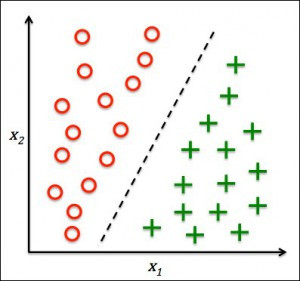
\includegraphics[width = 0.3\linewidth]{figures/04/01_classification/classification_motivation.jpg}
\end{figure}
\textbf{Classification} is the problem of identifying to which of a set of categories (sub-populations) a new observation belongs (e.g. assigning a given email into "spam" or "non-spam").
\newline
Qualitative response variables (categorical)
\begin{itemize}
\item Mean/median cannot be defined
\item No meaningful ordering
\end{itemize}
\end{frame}
\begin{frame}
\frametitle{classification algorithms}
There are many algorithms that can learn how to do classification
\begin{itemize}
\item decision trees
\item random forests
\item support vector machines
\item logistic regression
\item artificial neural network
\item ...
\end{itemize}
\end{frame}



\section{decision tree}
\begin{frame}
\frametitle{motivation}
How can we create such a decision tree using data?
\begin{figure}
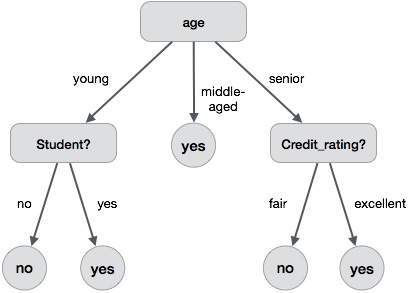
\includegraphics[width = 0.6\linewidth]{figures/04/01_classification/decision_tree_rating.jpg}
\end{figure}
\end{frame}
\subsection{induction algorithm}
\begin{frame}
\frametitle{overview}
Decision tree builds classification 

\begin{itemize}
\item in form of a tree structure
\item breaks down a dataset into smaller and smaller subsets while at the same time an associated decision tree is incrementally developed. The final result is a tree with decision nodes and leaf nodes. 
\item A decision node (e.g., Outlook) has two or more branches (e.g., Sunny, Overcast and Rainy). Leaf node (e.g., Play) represents a classification or decision.
\item The topmost decision node in a tree which corresponds to the best predictor called root node.
\end{itemize}
\end{frame}
\begin{frame}
\frametitle{induction(1)}
A decision tree is built top-down:
\begin{itemize}
\item starting from a root node
\item partition each node so that the following nodes are maximal "pure"/homogeneous nudes (contain instances with similar values)
\item if the node is maximal pure: stop induction and assign label
\end{itemize}
\end{frame}


\begin{frame}
\frametitle{induction}
Splitting the data while going through the decision tree:
\begin{figure}
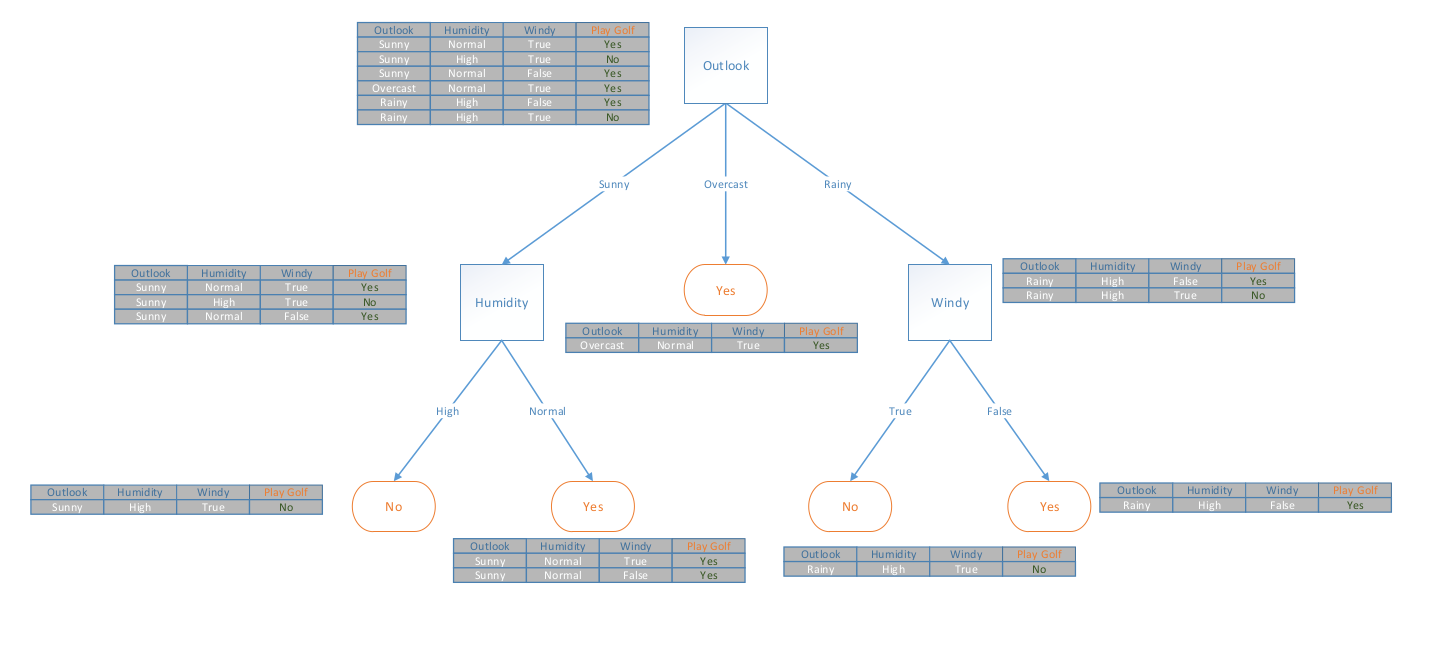
\includegraphics[width = 1.0\linewidth]{figures/04/01_classification/decision_tree_induction.png}
\end{figure}
\end{frame}


\begin{frame}
\frametitle{information measures(1)}
How can we know, which attribute should be splitted at a node?
\newline
\textbf{idea:} select at a given node $v$ the attribute that minimizes the "impurity" in its following nodes.
\newline
Now we have to formalize impurity of a node:
\begin{itemize}
\item entropy
\item gini coefficient
\item ...
\end{itemize}
We will focus on entropy since it is the most prominent measure in decision tree induction:
\begin{block}{entropy}
$entropy(v) = -\sum_{i} p_i log_2(p_i)$
\end{block}
$p_i$ is the probability/relative frequency of class $i$ in node $v$
\end{frame} 

\begin{frame}
\frametitle{information measures (2)}
\begin{figure}
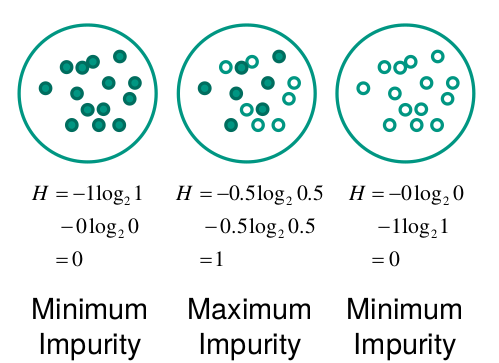
\includegraphics[width = 0.5\linewidth]{figures/04/01_classification/entropy.png}
\end{figure}


\end{frame}

\begin{frame}
\frametitle{information measures (3)}
We calculate the impurity for each attribute at each node. We want the impurity of father and subnodes to be maximal. The so called information gain describes how much impurity we can remove when splitting with attribute $a$ into $k$ subnodes:
\begin{block}{information gain}
$informationGain(a,v) = entropy(v) - \sum_k \frac{n_k}{n} entropy(k)$
\end{block}
$n_k$ is the number of observations in subnode $k$
\newline
$n$ is the number of observations in the father node $v$
\end{frame}

\begin{frame}
\frametitle{example}
\begin{figure}
\centering
\begin{minipage}{.4\textwidth}
Information gain tells us \newline
how good the given split \newline on an
attribute is
\begin{figure}
  \centering
  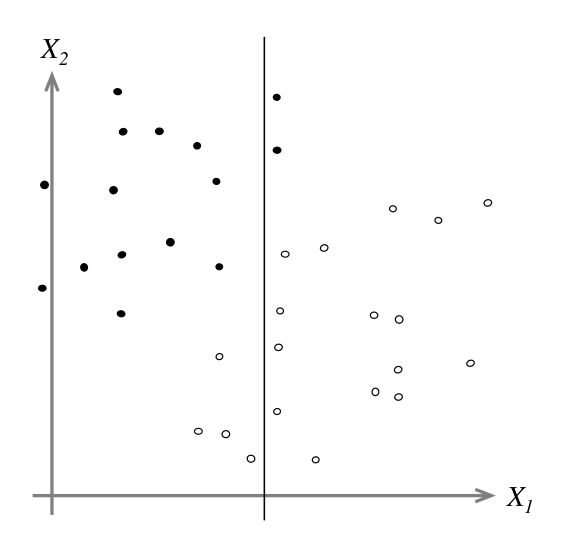
\includegraphics[width=1\linewidth]{figures/04/01_classification/example_decision.png}
\end{figure}
Information gain: 
\newline
$0.989 - 0. 655=0.334$


\end{minipage}%
\begin{minipage}{.5\textwidth}
Entire population (34 instances)
„parent entropy“:
\newline
$- \frac{15}{34} log_2 (\frac{15}{34})-\frac{19}{34} log_2 (\frac{19}{34}) = 0.989 $
\newline
\newline
"child entropy" of left side (17 instances):
\newline
$- \frac{13}{17} log_2 (\frac{13}{17})-\frac{4}{17} log_2 (\frac{4}{17}) = 0.787 $
\newline
\newline
"child entropy" of right side (17 instances):
\newline
$- \frac{2}{17} log_2 (\frac{2}{17})-\frac{15}{17} log_2 (\frac{15}{17}) = 0.523$
\newline
\newline
Entropy of children:
\newline
$\frac{17}{34} 0.787 + \frac{17}{34} 0.523 = 0.655$
\end{minipage}
\end{figure}
\end{frame}


\begin{frame}
\frametitle{example}
\begin{figure}
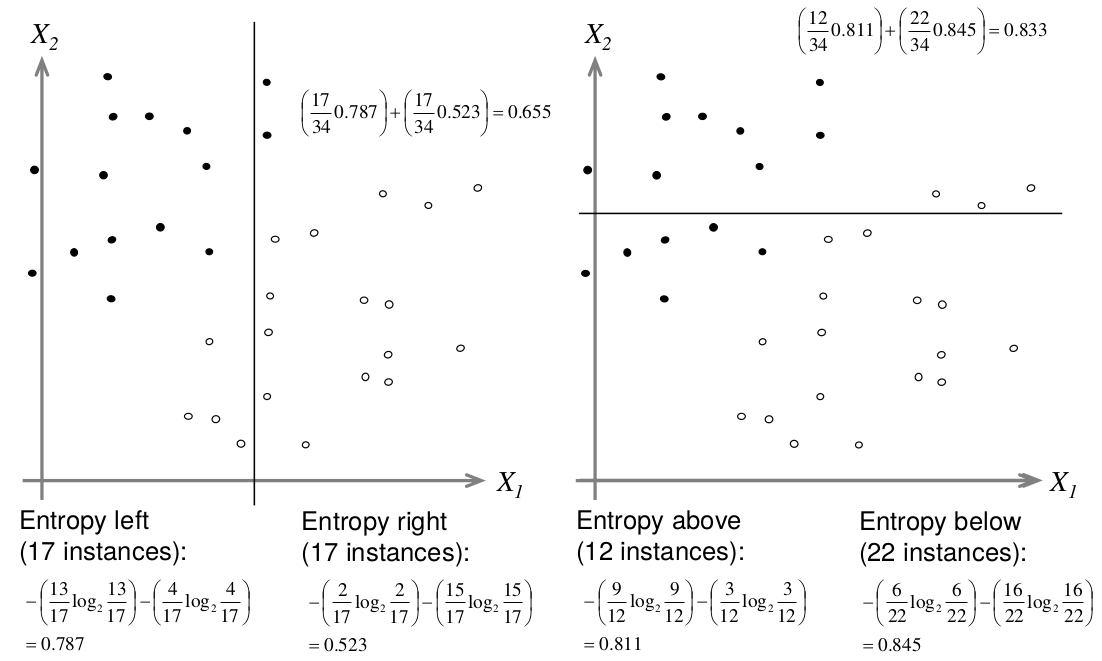
\includegraphics[width = 1\linewidth]{figures/04/01_classification/example_decision_2.png}
\end{figure}
\end{frame}

\begin{frame}
\frametitle{example}
\begin{figure}
\centering
\begin{minipage}{.5\textwidth}
\begin{figure}
  \centering
  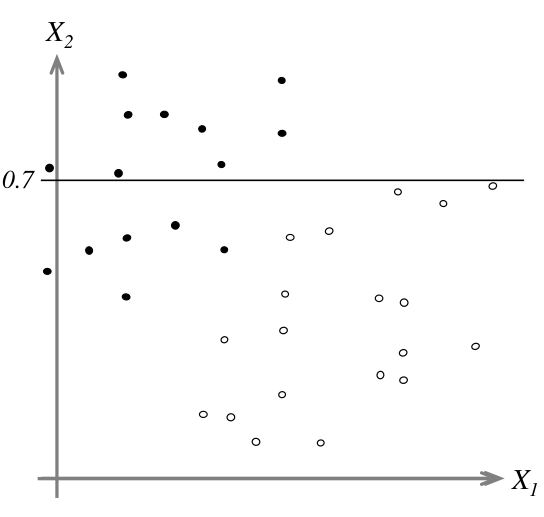
\includegraphics[width=.9\linewidth]{figures/04/01_classification/example_decision_3.png}
\end{figure}
Select the variable (here $X_2$ ) and
\newline
split (here at 0.7) that yields the
\newline
highest information gain
\end{minipage}%
\begin{minipage}{.5\textwidth}
\begin{figure}
  \centering
  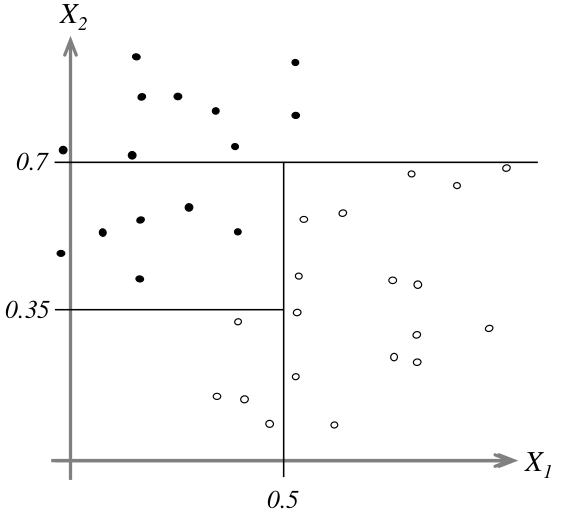
\includegraphics[width=.9\linewidth]{figures/04/01_classification/example_decision_4.png}
\end{figure}
Do this iteratively until no more
impurity exists (the set of points
is fully classified)
\end{minipage}
\end{figure}
\end{frame}

\begin{frame}
\frametitle{example}
\begin{figure}
\centering
\begin{minipage}{.5\textwidth}
Ultimately resulting in:
\begin{figure}
  \centering
  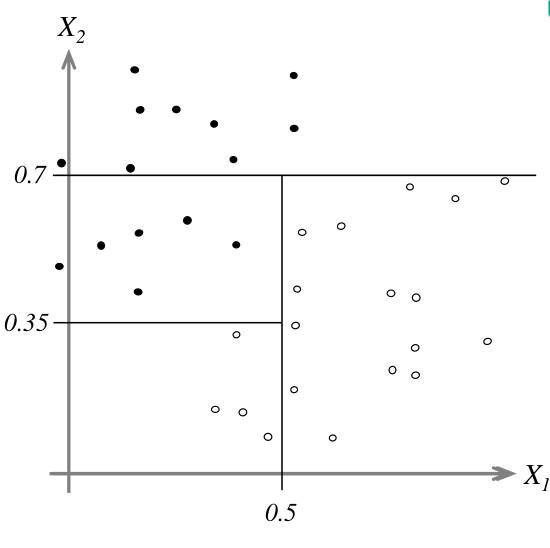
\includegraphics[width=.9\linewidth]{figures/04/01_classification/example_decision_5.png}
\end{figure}
\end{minipage}%
\begin{minipage}{.5\textwidth}
Corresponding decision tree:
\begin{figure}
  \centering
  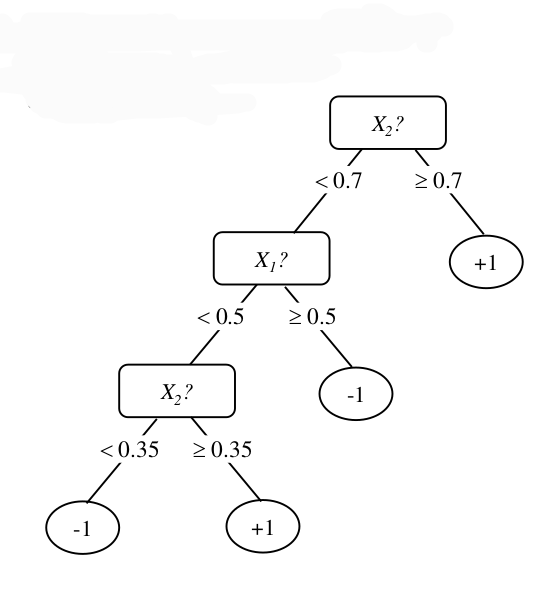
\includegraphics[width=.9\linewidth]{figures/04/01_classification/example_decision_6.png}
\end{figure}

\end{minipage}
\end{figure}
\end{frame}


\begin{frame}
\frametitle{pseudocode}
\begin{figure}
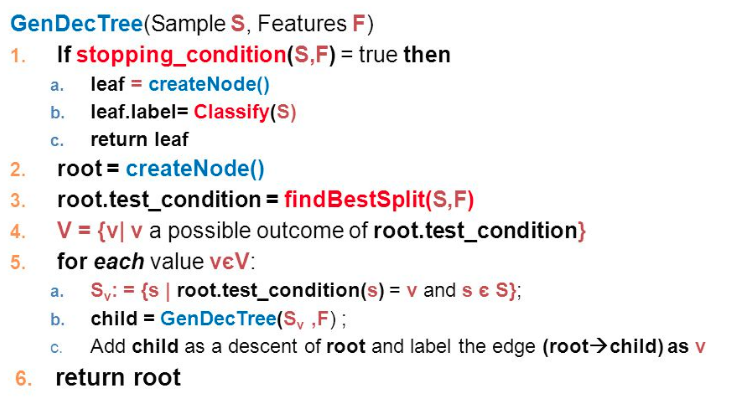
\includegraphics[width = 1\linewidth]{figures/04/01_classification/pseudocode.png}
%link: http://slideplayer.com/5260539/16/images/29/Constructing+decision-trees+%28pseudocode%29.jpg
\end{figure}
\end{frame}

\begin{frame}
\frametitle{pros \& cons of decision trees}
\begin{itemize}
\item easy to construct
\item very visual and interpretable model
\item not much predicting "power"
\item can be used for rule generation 
\item handling both continuous and discrete data
\item calculation growth when problem is getting bigger
\item tree might get too large
\end{itemize}
\end{frame}

\subsection{extensions: bagging, random forest}

\begin{frame}
\frametitle{random forest}
\begin{figure}
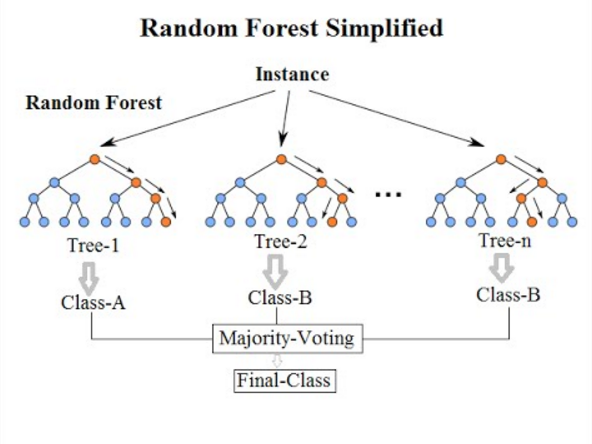
\includegraphics[width = 0.9\linewidth]{figures/04/01_classification/random_forest.png}
%link: https://cdn-images-1.medium.com/max/592/1*i0o8mjFfCn-uD79-F1Cqkw.png
\end{figure}

\end{frame}







\begin{frame}
\Huge{\centerline{The End}}
\end{frame}

%----------------------------------------------------------------------------------------

\end{document}